\chapter{Amazon Web Services}\label{chapter:kapitellabel} %%%%%%%%%%%%%%%%%%%%%%%%%%%%
Amazon Web Services (AWS) gehört zum amerikanischen Online-Versandhändler Amazon und beschreibt die
seit 2006 entwickelten Infrastrukturdienstleistungen, welche zu Beginn für andere Unternehmen angeboten
wurden und seit {{\color{red}2012 im Zuge der voranschreitenden Cloud-Computing-Technologie auch
privaten Nutzern angeboten werden} \cite{aws:general}. Ihren Ursprung haben die Dienste in den Bedürfnissen von Amazon selbst. Als Online-Versandhändler unterliegt das Unternehmen einem dynamischen
Nutzungsaufkommen. Gerade zu saisonalen Ereignissen wie Weihnachten sind die Anfragen
an die Webseiten und damit an die bereitgestellten IT-Ressourcen gut zehnmal höher als
in der restlichen Zeit des Jahres. Damit die Ressourcen in dieser Zeit nicht ungenutzt
bleiben und nur Geld kosten, entstand die Idee, die freien Kapazitäten an Dritte zu verkaufen.
Dabei nutzt Amazon den Pooling-Effekt: Ungenutzte Ressourcen landen in einem gedachten Pool und
können je nach Bedarf weitergenutzt werden. Hierdurch gelingt es Amazon ein für Nutzer
sehr attraktives Modell zu schaffen, durch welches sie sich je nach Bedarf flexible
Ressourcen und Kapazitäten zusammenstellen können \cite{baun:springer}.

Cloud-Bezug und Klassifizierungen

Gruppierung der Dienste nach Amazon (sind ganz schön viele weil AWS ziemlich wächst, daher die gängigsten)

Die entwickelten Dienstleistungen beinhalten die Bereitstellung von Servern sowie
zugehörigen Diensten, Speicherplatz, Datenbanken und Anwendungsservices wie zum
Beispiel Cloud Search, eine skalierbare Suchfunktionalität in Anwendungen, oder
den “Desktop in der Cloud” mit Workspaces. Amazon betreibt und verwaltet dabei
die über ein Netzwerk miteinander verbundene Hardware, welche für die korrekte
Funktion der Anwendungsservices benötigt wird, sowie die benötigten Ressourcen,
welche über eine Webanwendung bereitgestellt und genutzt werden. Mit seinem Angebot
zählt AWS zu den bedeutendsten internationalen Angeboten im Cloud Computing.

\section{Regions}
\section{Vorteile}
\section{Kosten}
\section{Sicherheit}

  See \ref{figure:helloworld}.

\begin{figure}[!ht] % see https://en.wikibooks.org/wiki/LaTeX/Floats,_Figures_and_Captions for placement parameters
  \centering
  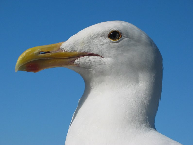
\includegraphics[width=0.5\textwidth]{images/gull.png}
  \caption{A picture of a gull.}
\end{figure}

Lorem ipsum dolor sit amet, consectetur adipiscing elit, sed do eiusmod tempor incididunt ut labore et dolore magna aliqua. Ut enim ad minim veniam, quis nostrud exercitation ullamco laboris nisi ut aliquip ex ea commodo consequat. Duis aute irure dolor in reprehenderit in voluptate velit esse cillum dolore eu fugiat nulla pariatur. Excepteur sint occaecat cupidatat non proident, sunt in culpa qui officia deserunt mollit anim id est laborum

Lorem ipsum dolor sit amet, consectetur adipiscing elit, sed do eiusmod tempor incididunt ut labore et dolore magna aliqua. Ut enim ad minim veniam, quis nostrud exercitation ullamco laboris nisi ut aliquip ex ea commodo consequat. Duis aute irure dolor in reprehenderit in voluptate velit esse cillum dolore eu fugiat nulla pariatur. Excepteur sint occaecat cupidatat non proident, sunt in culpa qui officia deserunt mollit anim id est laborum

Lorem ipsum dolor sit amet, consectetur adipiscing elit, sed do eiusmod tempor incididunt ut labore et dolore magna aliqua. Ut enim ad minim veniam, quis nostrud exercitation ullamco laboris nisi ut aliquip ex ea commodo consequat.
\begin{figure}[H]
  \centering
  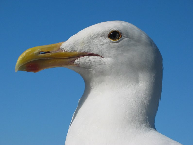
\includegraphics[width=0.5\textwidth]{images/gull.png}
  \caption{A picture of a gull.}
\end{figure}
Duis aute irure dolor in reprehenderit in voluptate velit esse cillum dolore eu fugiat nulla pariatur. Excepteur sint occaecat cupidatat non proident, sunt in culpa qui officia deserunt mollit anim id est laborum

Lorem ipsum dolor sit amet, consectetur adipiscing elit, sed do eiusmod tempor incididunt ut labore et dolore magna aliqua. Ut enim ad minim veniam, quis nostrud exercitation ullamco laboris nisi ut aliquip ex ea commodo consequat. Duis aute irure dolor in reprehenderit in voluptate velit esse cillum dolore eu fugiat nulla pariatur. Excepteur sint occaecat cupidatat non proident, sunt in culpa qui officia deserunt mollit anim id est laborum


% keep an blank line above
